%============================================================
% DEMO — Beamer + metropolis  (LaTeX modernizado)
% Compilar:  xelatex demo.tex   (metropolis usa fuentes Fira;
%            con pdflatex también funciona pero se ve mejor con xelatex)
%============================================================
\documentclass[11pt,aspectratio=169]{beamer}

\usetheme{metropolis}
\metroset{block=fill, numbering=fraction, progressbar=frametitle}

\usepackage{amsmath, amssymb}
\usepackage{graphicx}
\graphicspath{{../../images/}}   % apunta a la carpeta de figuras de la tesis

% Color de acento (puedes cambiarlo por el institucional de la UdeC)
\definecolor{udecblue}{RGB}{0,70,140}
\setbeamercolor{frametitle}{bg=udecblue}
\setbeamercolor{progress bar}{fg=udecblue}

\title{Deep Learning para problemas de información cuántica}
\subtitle{Defensa de Tesis Doctoral --- \textit{demo Beamer + metropolis}}
\author{Antonio Guerra}
\institute{Universidad de Concepción}
\date{\today}

\begin{document}

\maketitle

%------------------------------------------------------------
\begin{frame}{Hoja de ruta}
  \begin{enumerate}
    \item \textbf{Background} --- información cuántica y deep learning
    \item \textbf{Estado del arte} --- combinando ambos mundos
    \item \textbf{Contribución 1} --- interpolación de unitarias (PINNs)
    \item \textbf{Contribución 2} --- reconstrucción desde marginales (CDAE + MIO)
    \item \textbf{Conclusiones} y trabajo futuro
  \end{enumerate}

  \vspace{1em}
  \begin{alertblock}{Idea rectora}
    Incrustar la física conocida en el aprendizaje (\emph{physics-informed})
    extiende los métodos clásicos a problemas cuya complejidad crece como $2^N$.
  \end{alertblock}
\end{frame}

%------------------------------------------------------------
\begin{frame}{Background: la barrera exponencial}
  \begin{columns}[T]
    \begin{column}{0.55\textwidth}
      Un estado de $N$ qubits vive en un espacio de dimensión $2^N$:
      \[
        \rho(t) = U(t)\,\rho_0\,U^{\dagger}(t), \qquad
        i\,\dot U = H(t)\,U .
      \]
      \begin{itemize}
        \item Construir/exponenciar $U(t)$ escala como $\mathcal{O}(2^{3N})$.
        \item Con $H(t)$ dependiente del tiempo no hay $e^{-iHt}$ cerrado.
      \end{itemize}
    \end{column}
    \begin{column}{0.45\textwidth}
      \begin{block}{Physics-informed learning}
        La física entra por la \emph{loss}: la red aprende solo soluciones
        físicamente admisibles (unitaridad, positividad, marginales).
      \end{block}
    \end{column}
  \end{columns}
\end{frame}

%------------------------------------------------------------
\begin{frame}{Contribución 1 --- Interpolación de unitarias con PINNs}
  \begin{columns}[c]
    \begin{column}{0.5\textwidth}
      Dada $U(t_i)$ en tiempos muestreados, interpolar $U(t)$ en todo $[0,T]$
      \textbf{sin conocer el Hamiltoniano}.
      \[
        F\big(U,U_\theta\big) =
        \left| \tfrac{1}{d}\,\mathrm{Tr}\!\left[U^{\dagger}U_\theta\right]\right|^2
      \]
      \begin{itemize}
        \item Fidelidad $\approx 0.99$ (2--8 qubits)
        \item Speedups $8.9\times$--$19.3\times$ vs.\ geodésica
      \end{itemize}
    \end{column}
    \begin{column}{0.5\textwidth}
      \centering
      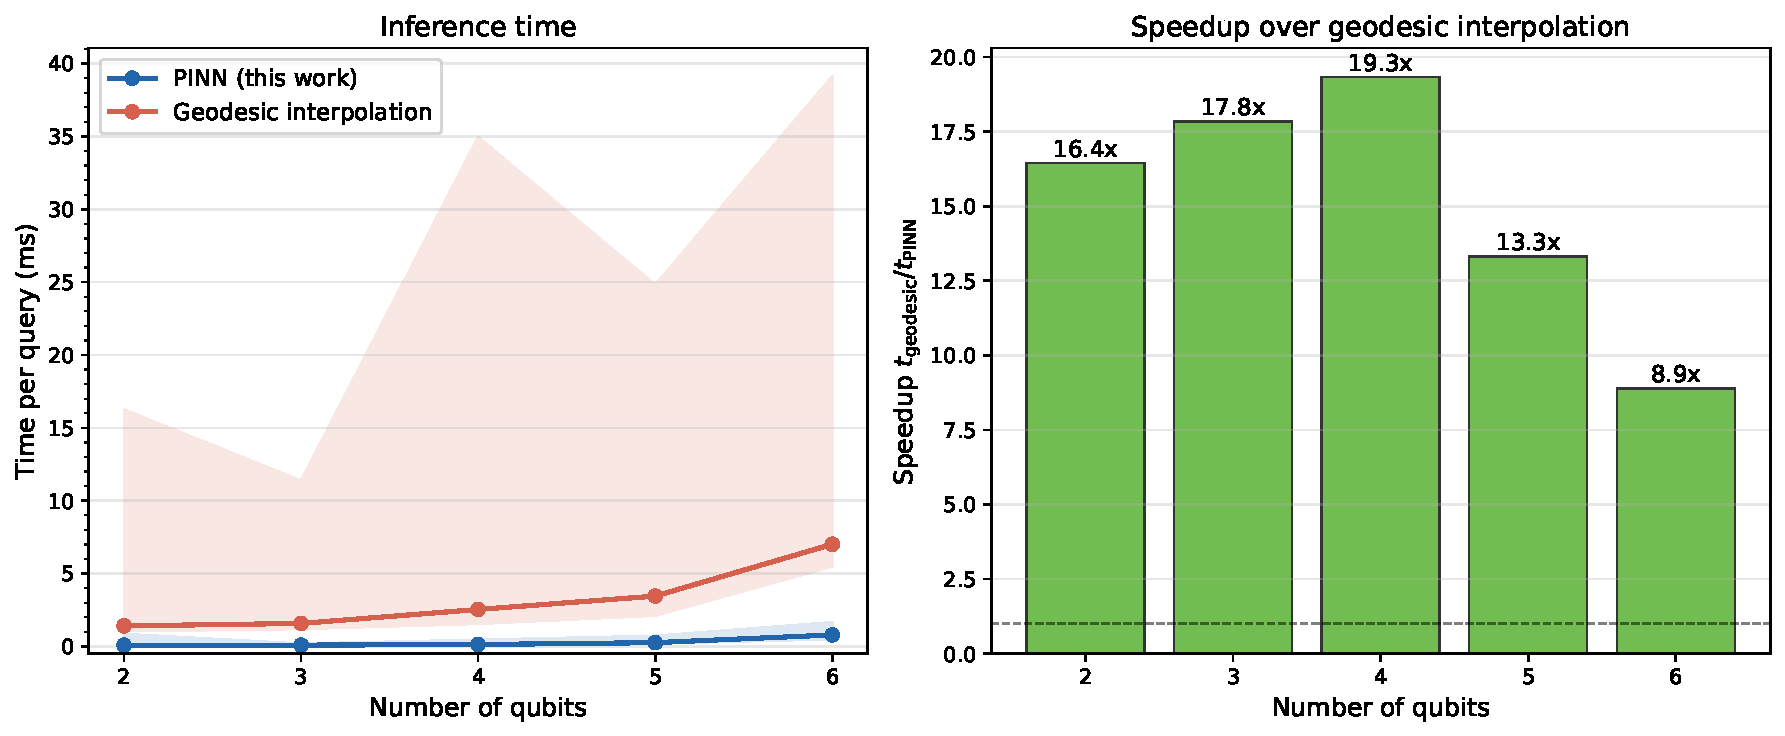
\includegraphics[width=\linewidth]{timing_benchmark.pdf}
    \end{column}
  \end{columns}
\end{frame}

%------------------------------------------------------------
\begin{frame}{Contribución 2 --- Reconstrucción desde marginales (CDAE + MIO)}
  \begin{columns}[c]
    \begin{column}{0.5\textwidth}
      El \emph{Quantum Marginal Problem} (QMA-completo): dado
      $\{\sigma_{\mathcal{J}}\}$, reconstruir un estado global $\rho$ compatible.
      \begin{itemize}
        \item Matriz de densidad $\to$ imagen de 2 canales
        \item CDAE + MIO $\to$ estado físico válido
        \item \textbf{Transfer learning} de 3 a 8 qubits
        \item Más rápido que SDP (resuelve donde SDP falla)
      \end{itemize}
    \end{column}
    \begin{column}{0.5\textwidth}
      \centering
      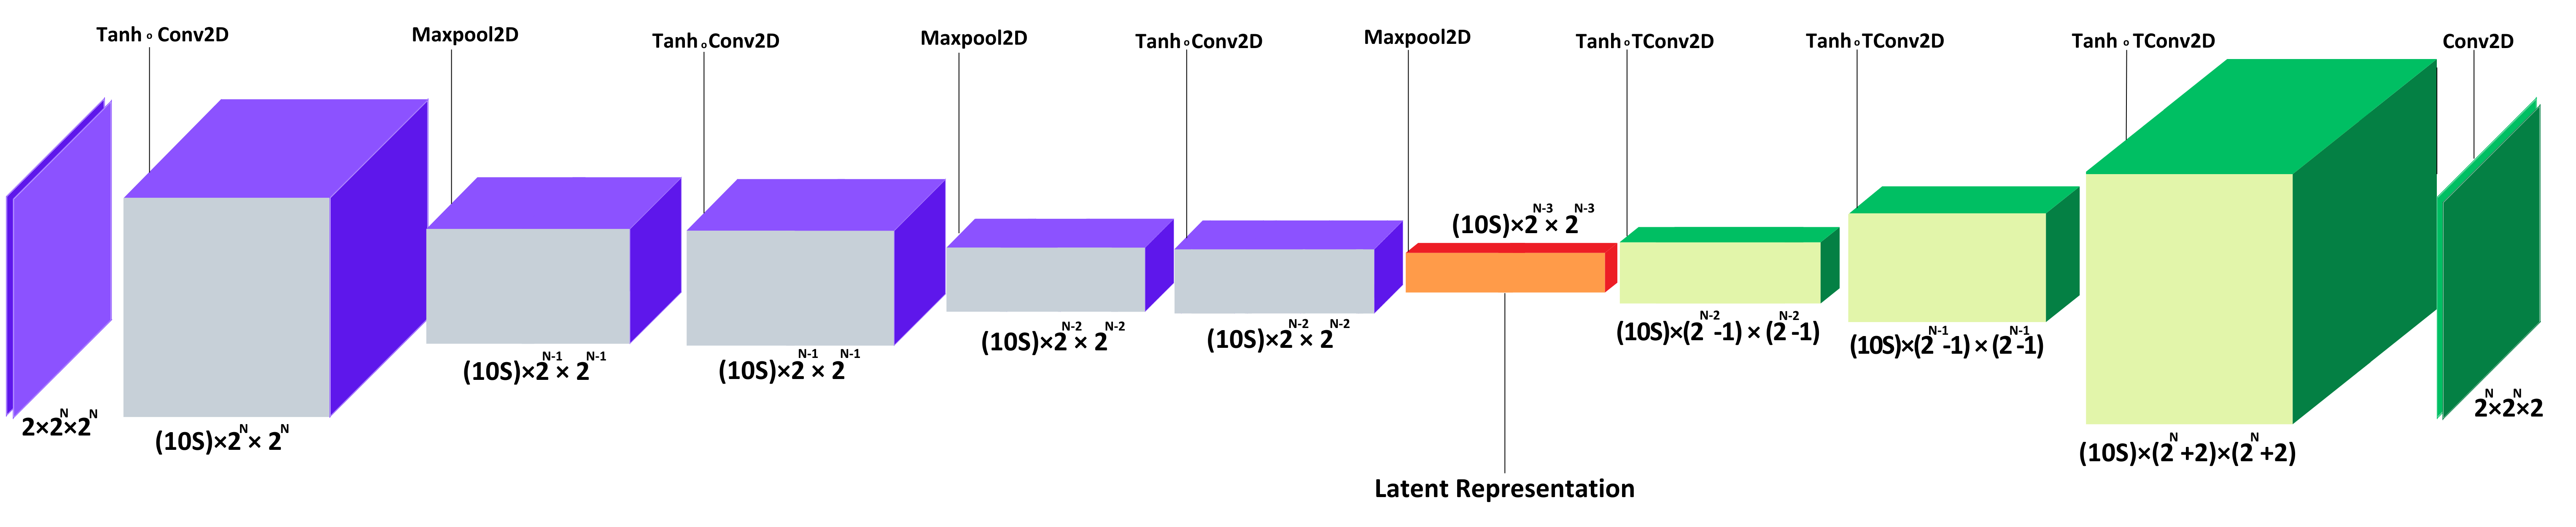
\includegraphics[width=\linewidth]{DA_architecture.png}
    \end{column}
  \end{columns}
\end{frame}

%------------------------------------------------------------
\begin{frame}[standout]
  Dos problemas duros, un mismo patrón:\\
  \alert{la física en la loss} convierte lo intratable en aprendible.
\end{frame}

\end{document}
